\begin{frame}{La placa de desarrollo MOJO v3}
	\begin{columns}
		\begin{column}{.43\textwidth}
			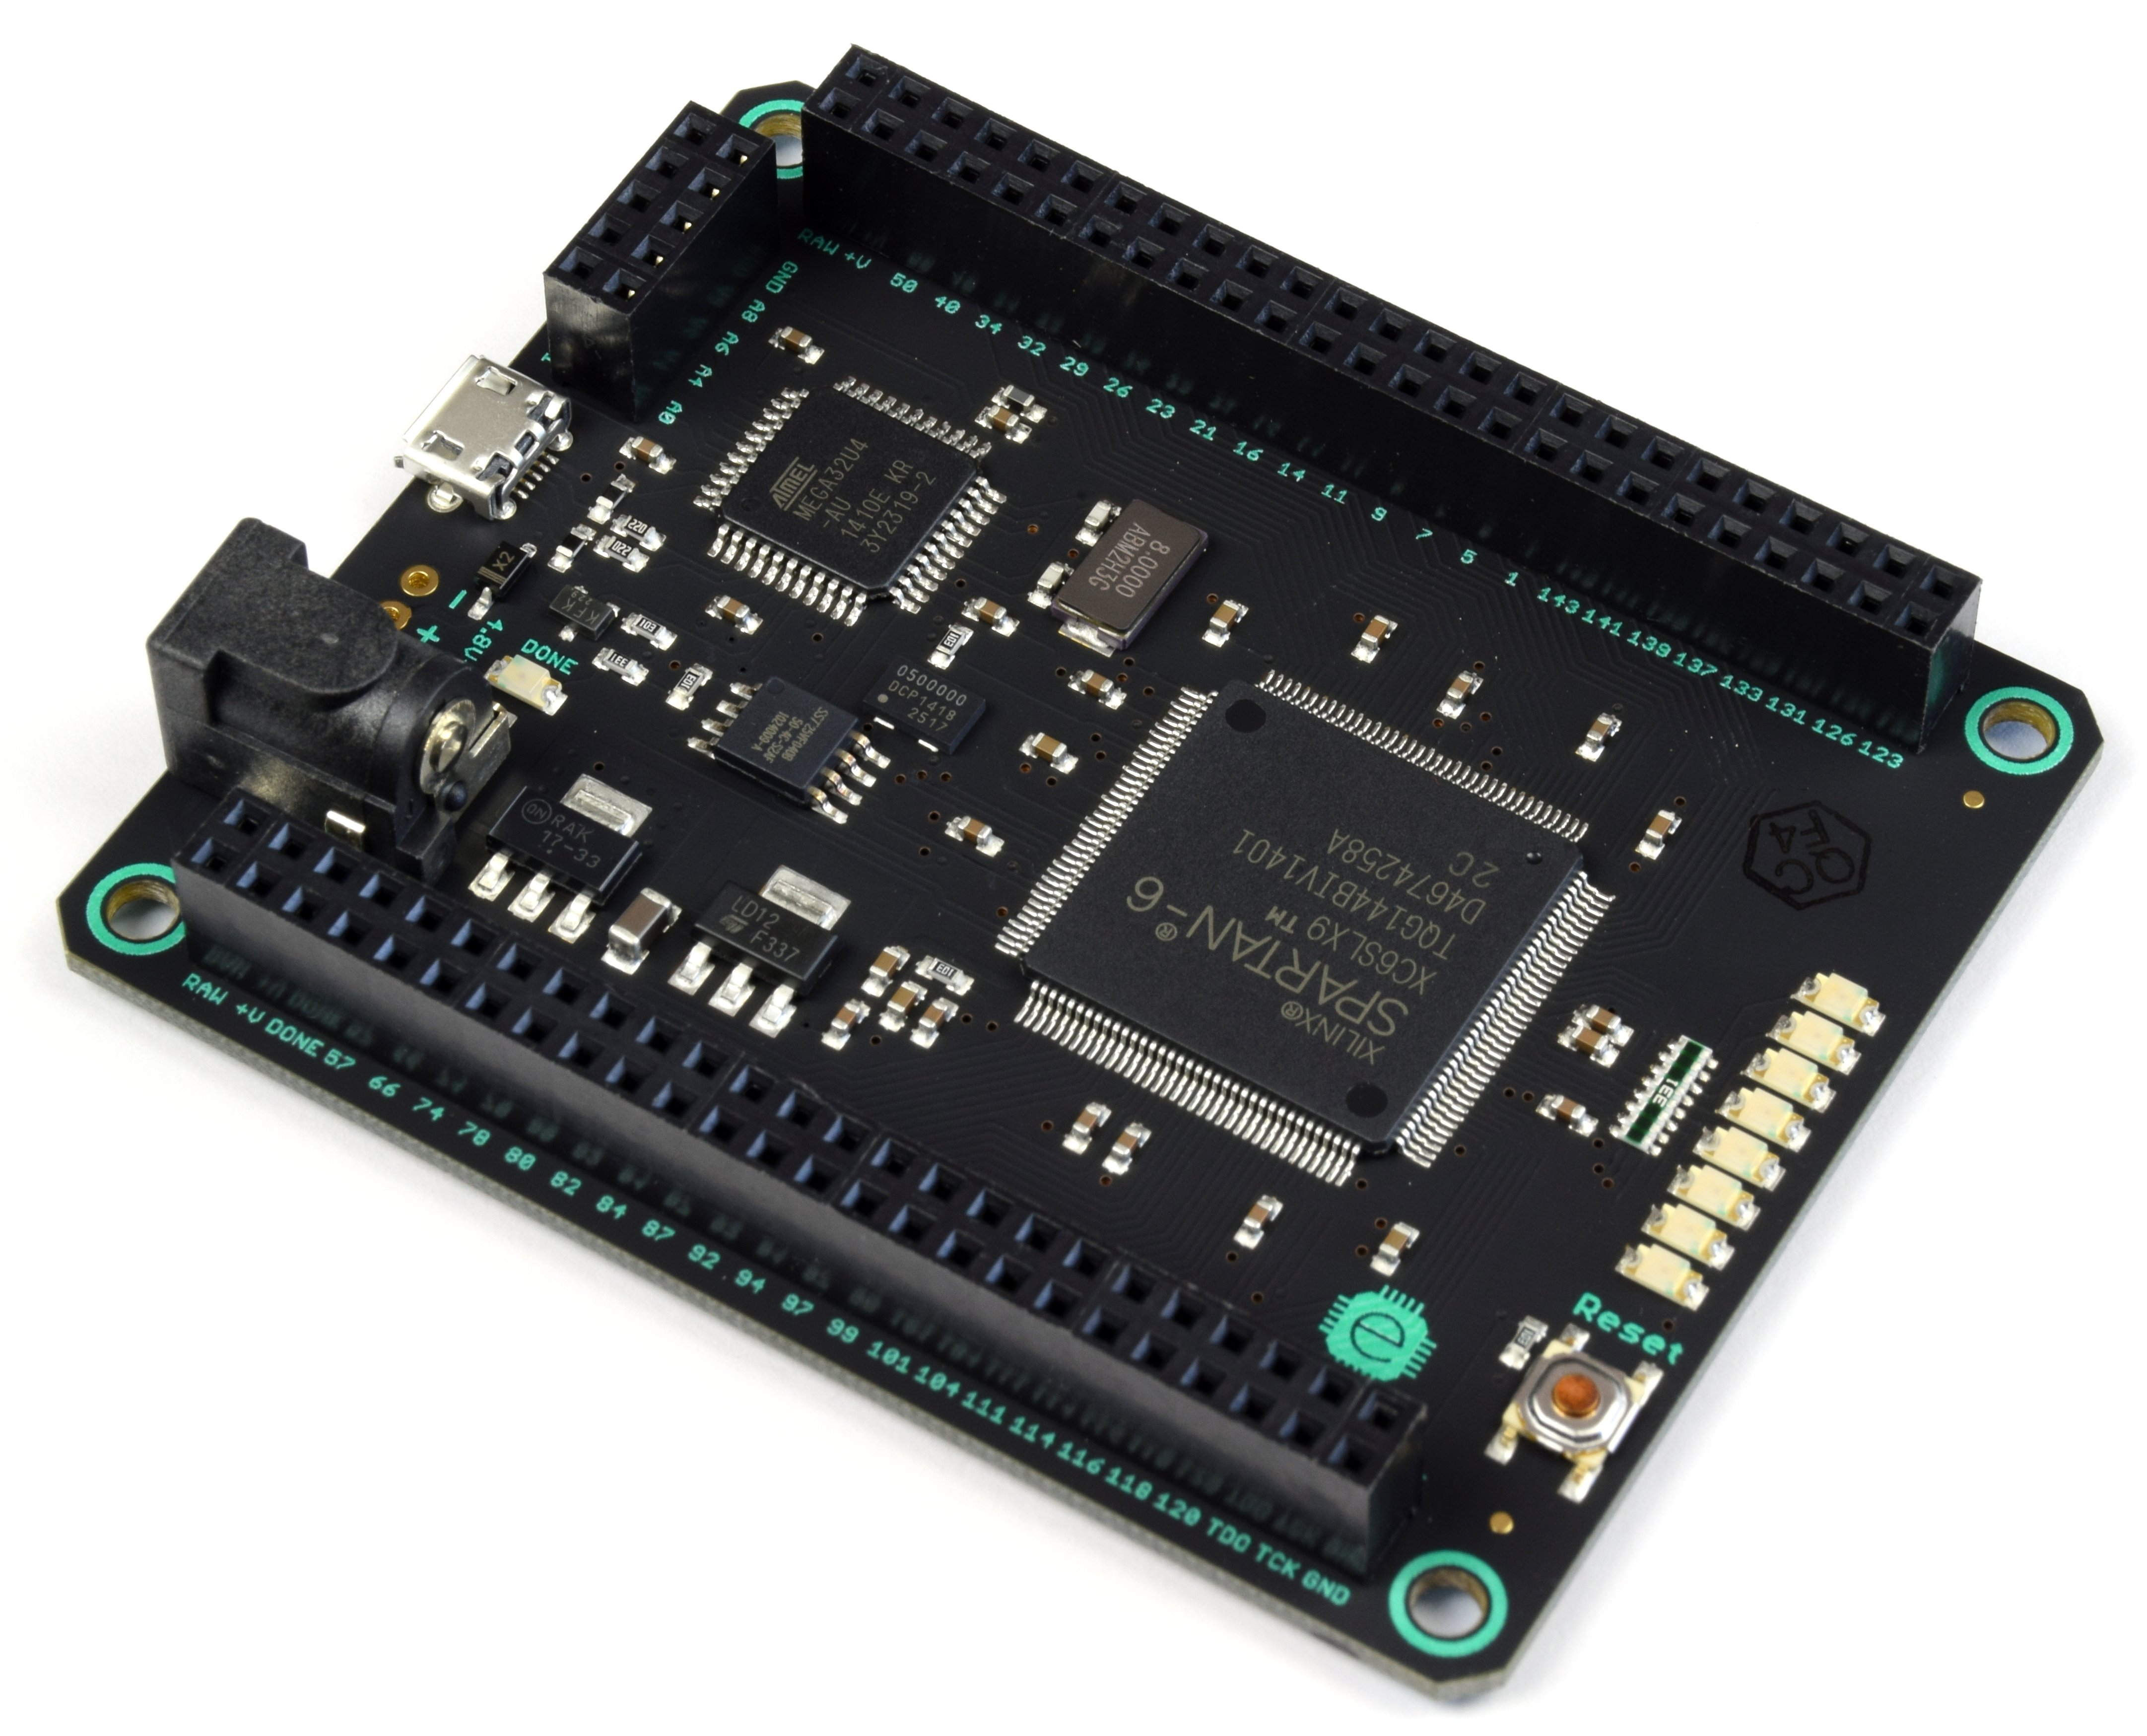
\includegraphics[width=\textwidth]{MojoIso.png}
		\end{column}
		\begin{column}{.55\textwidth}
			\begin{itemize}
				\item FPGA Spartan 6 XC6SLX9 de Xilinx
				\item 84 pines IO digitales
				\item 8 entradas analógicas
				\item 8 LEDs de propósito general
				\item 1 pulsador de propósito general
				\item Regulador de voltaje de entrada de 4.8V - 12V
				\item ATmega32U4 para configurar la FPGA y leer los pines analógicos
				\item Bootloader compatible con Arduino
				\item Memoria flash para almacenar la configuración de la FPGA (programación persistente)
			\end{itemize}
		\end{column}
	\end{columns}
\end{frame}
\begin{frame}{Estructura interna FPGA}
	\centering
	\begin{tikzpicture}[scale=.58]
		\begin{scope}[transform shape,node distance=5,>=latex,thick]
			\node[simple]	(cypress)		[]	 			{FIFO Esclava};
			\node[simple]	(master)	[right=of cypress]	{Maestro Externo};
			\node[simple,minimum size=70]	(leer)		[right=of master.north west,anchor=north west] {Leer FIFO};
			\node[simple,minimum size=70]	(escribir)	[right=of master.south west,anchor=south west]	{Escribir FIFO};
			\node[simple,node distance=8]	(fifo)		[right=of master]	{FIFO Interna (XLNX core generator)};
			
			\draw[<->]	([yshift=4*110/6]cypress.east) --node [above]{IFCLK} ([yshift=4*110/6]master.west);
			\draw[<->]	([yshift=3*110/6]cypress.east) --node [above]{FD[15:0]} ([yshift=3*110/6]master.west);
			\draw[<-]	([yshift=2*110/6]cypress.east) --node [above]{FIFOADR[1:0]} ([yshift=2*110/6]master.west);
			\draw[->]	([yshift=1*110/6]cypress.east) --node [above]{EP2\_EMPTY} ([yshift=1*110/6]master.west);
			\draw[->]	([yshift=0*110/6]cypress.east) --node [above]{EP8\_FULL} ([yshift=0*110/6]master.west);
			\draw[<-]	([yshift=-1*110/6]cypress.east) --node [above]{SLOE} ([yshift=-1*110/6]master.west);
			\draw[<-]	([yshift=-2*110/6]cypress.east) --node [above]{SLWR} ([yshift=-2*110/6]master.west);
			\draw[<-]	([yshift=-3*110/6]cypress.east) --node [above]{SLRD} ([yshift=-3*110/6]master.west);
			\draw[<-]	([yshift=-4*110/6]cypress.east) --node [above]{PKTEND} ([yshift=-4*110/6]master.west);
			
			\draw[<-] (leer) -- node[above]{SLWR} (master.east |- leer);
			\draw[<-] ([yshift=-1*80/7]leer.east) -- node[above]{EMPTY}([yshift=-1*80/7]fifo.west |- leer);
			\draw[->] ([yshift=1*80/7]leer.east) -- node[above]{RD\_EN}([yshift=1*80/7]fifo.west |- leer);
			
			\draw[<-] (escribir) -- node[above]{SLRD} (master.east |- escribir);
			\draw[<-] ([yshift=-1*80/7]escribir.east) -- node[above]{FULL}([yshift=-1*80/7]fifo.west |- escribir);
			\draw[->] ([yshift=1*80/7]escribir.east) -- node[above]{WR\_EN}([yshift=1*80/7]fifo.west |- escribir);			
			
			\draw[<-]	([yshift=1*110/6]fifo.west) --node [above]{DIN[15:0]} ([yshift=1*110/6]master.east);
			\draw[->]	([yshift=0*110/6]fifo.west) --node [above]{DOUT[15:0]} ([yshift=0*110/6]master.east);
			\draw[<-]	([yshift=-1*110/6]fifo.west) --node [above]{VALID} ([yshift=-1*110/6]master.east);
			
			\node[node distance=.4] (fpga) [above=of leer] {FPGA};
		\end{scope}
		\begin{scope}[on background layer]
			\node[rectangle,rounded corners,dashed,fit=(master)(leer)(fpga)(fifo)(escribir),draw=black]{};
		\end{scope}
	\end{tikzpicture}
\end{frame}
\begin{frame}{Interfaz - FPGA}
	\centering
	\begin{tikzpicture}[scale=.95]
		\begin{scope}[transform shape,node distance=5,>=latex]
			\node[simple]	(fifo)		[]	 			{FIFO Esclava};
			\node[simple]	(master)	[right=of fifo]	{Maestro Externo};
			\draw[<->,thick]	([yshift=5*110/6]fifo.east) --node [above]{IFCLK} ([yshift=5*110/6]master.west);
			\draw[<->,thick]	([yshift=4*110/6]fifo.east) --node [above]{FD[15:0]} ([yshift=4*110/6]master.west);
			\draw[<-,thick]	([yshift=3*110/6]fifo.east) --node [above]{FIFOADR[1:0]} ([yshift=3*110/6]master.west);
			\draw[->,thick]	([yshift=2*110/6]fifo.east) --node [above]{FLAGA} ([yshift=2*110/6]master.west);
			\draw[->,thick]	([yshift=1*110/6]fifo.east) --node [above]{FLAGB} ([yshift=1*110/6]master.west);
			\draw[->,thick]	([yshift=0*110/6]fifo.east) --node [above]{FLAGC} ([yshift=0*110/6]master.west);
			\draw[->,thick]	([yshift=-1*110/6]fifo.east) --node [above]{FLAGD} ([yshift=-1*110/6]master.west);
			\draw[<-,thick]	([yshift=-2*110/6]fifo.east) --node [above]{SLOE} ([yshift=-2*110/6]master.west);
			\draw[<-,thick]	([yshift=-3*110/6]fifo.east) --node [above]{SLWR} ([yshift=-3*110/6]master.west);
			\draw[<-,thick]	([yshift=-4*110/6]fifo.east) --node [above]{SLRD} ([yshift=-4*110/6]master.west);
			\draw[<-,thick]	([yshift=-5*110/6]fifo.east) --node [above]{PKTEND} ([yshift=-5*110/6]master.west);
		\end{scope}
	\end{tikzpicture}
\end{frame}
\begin{frame}{Operaciones con la FIFO - Lectura}
	contenidos...
\end{frame}
\begin{frame}{Máquina de estados algorítmica de la interfaz}
	\centering
	\begin{tikzpicture}[scale=.35]
		\begin{scope}[transform shape,node distance=1,>=latex]
			\node[moore]	(idle)	[]	{--idle:\\SLRD='1';\\SLOE='1';\\SLWR='1';\\FIFOADR="ZZ";};
			\node[ask]	(pr1)	[below=of idle]	{EP2\_empty='0'}
			edge[<-] (idle);
			\node[ask]	(pr2)	[right=of pr1]	{write\_req='1'};
			\node[ask]	(pr3)	[below=of pr2]	{EP8\_full='0'};
			\node[moore]	(radr)	[left=of pr1]		{--read address:\\SLRD='1';\\SLOE='1';\\SLWR='1';\\FIFOADR="00";};
			
			\draw[->](pr1) -- node [above,near start]{No}(radr);
			\draw[->](pr1) -- node [above,near start]{Si} (pr2);
			
			\node[node distance=0.8](aux1)[right=of pr2]{};
			\draw[->](pr2) -- node[left,near start]{Si}(pr3);
			\draw[->](pr2.east) |- node[above,near end]{No}(aux1.base);
			
			\node[moore]	(rnempty)	[left=of radr]	{--read no empty:\\SLRD='0';\\SLOE='0';\\SLWR='1';\\FIFOADR="00";}
			edge[<-](radr);
			\node[moore](rread)[below=of rnempty]{--read read:\\SLRD='1';\\SLOE='0';\\SLWR='1;\\FIFOADR="00";}
			edge[<-](rnempty);
			
			\node[moore](wadr)	[left=of pr3]	{--write address:\\SLRD='1';\\SLOE='1';\\SLWR='1';\\FIFOADR="11";};
			\node[node distance=.8](aux2)[right=of pr3]{};
			\draw[->](pr3) -- node[above,near start]{Si} (wadr);
			\draw[->](pr3) -- node[above,near start]{No}(aux2.base) -| (aux1.base);
			
			\node[moore](wnfull)[below=of wadr] {--write no full:\\SLRD='1';\\SLOE='1';\\SLWR='0';\\FIFOADR="11";}
			edge[<-] (wadr);
			\node[node distance=.5](aux3)[left=of wnfull]{};
			\draw[->] (wnfull) -- (aux3.base);
			\node[moore,node distance=.5](wwrite)[left=of aux3] {--write write:\\SLRD='1';\\SLOE='1';\\SLWR='1';\\FIFOADR="11";}
			edge[<-] (aux3.base);
			
			\node[ask](pr4)[below=of wwrite] {fifo\_valid='1'}
			edge[<-] (wwrite);
			\node[moore](wend)[left=of pr4] {--write end:\\SLRD='1';\\SLOE='1';\\SLWR='1';\\FIFOADR="11";};
			\node[node distance=.7] (aux4) [right=of pr4]{}; 
			\draw[->]	(pr4) -- node[above,near start]{Si} (wend);
			\draw[->](pr4) -- node[above] {No} (aux4.base);
			\draw[->](aux4.base) -- (aux3.base);
			
			\node[ask](pr5)[below=of wend] {write\_req='1'}
			edge[<-] (wend);
			\node[ask](pr6)[right=of pr5] {EP2\_empty='0'};
			\node[node distance=.8] (aux5) [left=of rread] {};
			\node[node distance=.8] (aux7) [left=of pr5] {};
			\draw[->] (rread) -- (aux5.base);
			\draw[->] (pr5)	-- node[above,near start] {No} (aux7.base);
			\draw[->] (pr5) -- node[above,near start] {Si} (pr6);
			
			\node[node distance=.8] (aux6)[below=of pr6] {};
			\draw[->] (pr6) -| node[above,near start] {Si} (wnfull);
			\draw[->] (pr6) -- node[left]{No} (aux6.base) -| (aux7.base);
			\draw[->] (aux7.base) |- (aux5.base);
			
			\node[node distance=.8] (aux8) [above=of idle] {};
			\draw[->] (aux8.base) -- (idle);
			\draw[->] (aux5.base) |- (aux8.base);
			\draw[->](aux1.base) |- (aux8.base);
			
		\end{scope}
	\end{tikzpicture}
\end{frame}
\begin{frame}{Maquinas de estado hacia la memoria FIFO interna}
	\begin{columns}
		\begin{column}{.5\textwidth}
			\centering
			\begin{tikzpicture}[scale=.53]
				\begin{scope}[transform shape,node distance=1,>=latex]
					\node[moore] (idle) {--idle:\\RE\_EN='0';};
					\node[node distance=.6](aux0)[above=of idle]{};
					\node[ask]	(pr1)	[below=of idle]{\tiny{SLWR='0'-$>$'1'}}
						edge[<-] (idle);
					\node[ask] (pr2) [below=of pr1]{\scriptsize{FIFO\_empty='1'}};
					\node[node distance=.8](aux1)[left=of pr1]{};
					\draw[->] (pr1) -- node[left] {Si} (pr2);
					\draw[->] (pr1) -- node[above,near start]{No} (aux1.base);
					\draw[->] (aux1.base) |- (aux0.base) -- (idle);
					
					\node[moore](rden)[below=of pr2]{--read enable:\\RD\_EN='1'};
					\node[node distance=.8] (aux2) [left=of pr2] {};
					\draw[->] (pr2) -- node[above,near start]{Si} (aux2.base);
					\draw[->] (pr2) -- node[left,near start] {No} (rden);
					\draw[->] (aux2.base) -- (aux1.base);
					
					\node[node distance=.8] (aux3) [below=of rden]{};
					\draw[->] (rden) -- (aux3.base) -| (aux2.base); 
				\end{scope}
			\end{tikzpicture}
		\end{column}
		\begin{column}{.5\textwidth}
			\centering
			\begin{tikzpicture}[scale=.5]
				\begin{scope}[transform shape,node distance=1,>=latex]
					\node[moore] (idle) {--idle:\\WR\_EN='0';};
					\node[node distance=.6](aux0)[above=of idle]{};
					\node[ask]	(pr1)	[below=of idle]{\tiny{SLRD='0'-$>$'1'}}
						edge[<-] (idle);
					\node[ask] (pr2) [below=of pr1]{\scriptsize{FIFO\_FULL='1'}};
					\node[node distance=.8](aux1)[left=of pr1]{};
					\draw[->] (pr1) -- node[left] {Si} (pr2);
					\draw[->] (pr1) -- node[above,near start]{No} (aux1.base);
					\draw[->] (aux1.base) |- (aux0.base) -- (idle);
					
					\node[moore](rden)[below=of pr2]{--write enable:\\WR\_EN='1'};
					\node[node distance=.8] (aux2) [left=of pr2] {};
					\draw[->] (pr2) -- node[above,near start]{Si} (aux2.base);
					\draw[->] (pr2) -- node[left,near start] {No} (rden);
					\draw[->] (aux2.base) -- (aux1.base);
					
					\node[node distance=.8] (aux3) [below=of rden]{};
					\draw[->] (rden) -- (aux3.base) -| (aux2.base); 
				\end{scope}
			\end{tikzpicture}
		\end{column}
	\end{columns}
\end{frame}
